% topic: Diffusion Models for Image Generation in Remote Sensing

\begin{frame}{\LARGE 目录}
  \begin{itemize}
    \item {\Large 背景:图像生成的生成式模型}
    \item {\Large 扩散模型:原理}
    \item {\Large 遥感中的应用}
    \item {\Large 总结和思考}
  \end{itemize}
\end{frame}


\begin{refsection}
  \begin{frame}
    \centering
    \vspace{2.5cm}
    {\LARGE \textbf{背景:图像生成的生成式模型}}
  \end{frame}
\end{refsection}

\begin{refsection}
  \begin{frame}{背景:图像生成的生成式模型}
    \begin{figure}
      \centering
      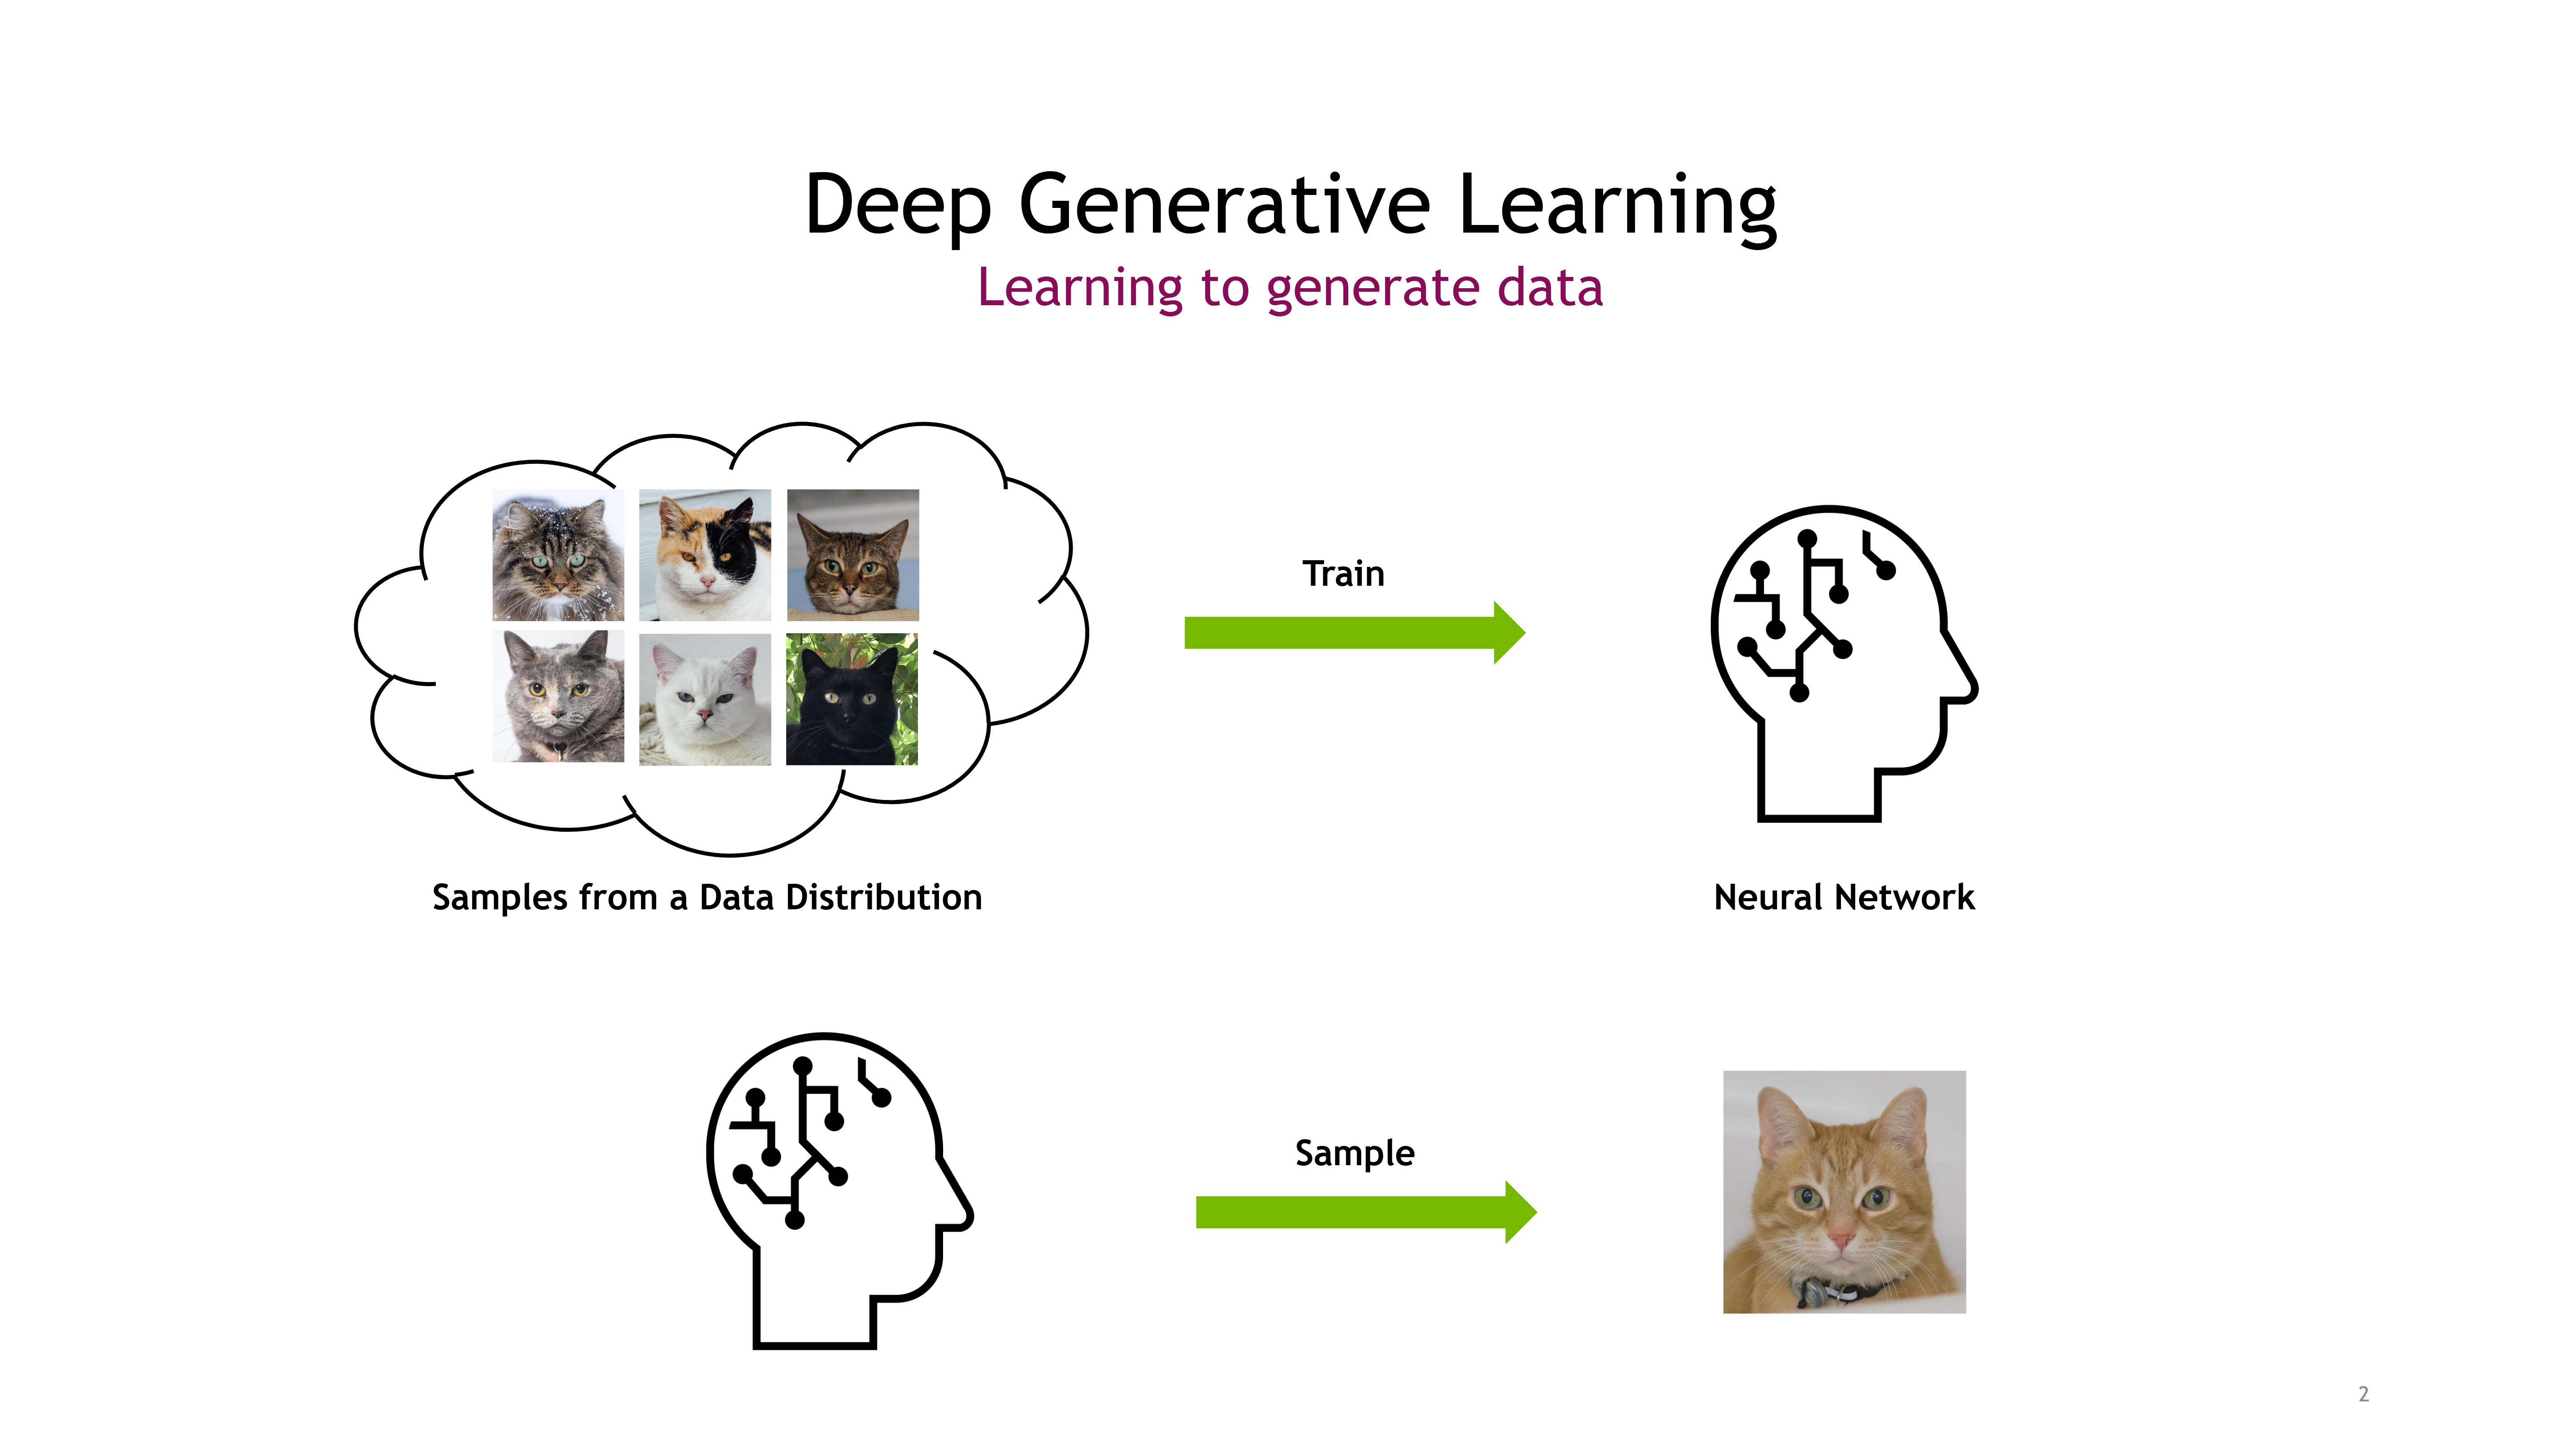
\includegraphics[width=0.8\linewidth]{learning_to_generate_data.png}
      \caption{\scriptsize 生成式建模示意图~\parencite{CVPR2023Tutorial}。}
    \end{figure}
    
    \bottomleftrefs
  \end{frame}
\end{refsection}

\begin{refsection}
  \begin{frame}{生成式模型发展时间线}
    \begin{figure}
      \centering
      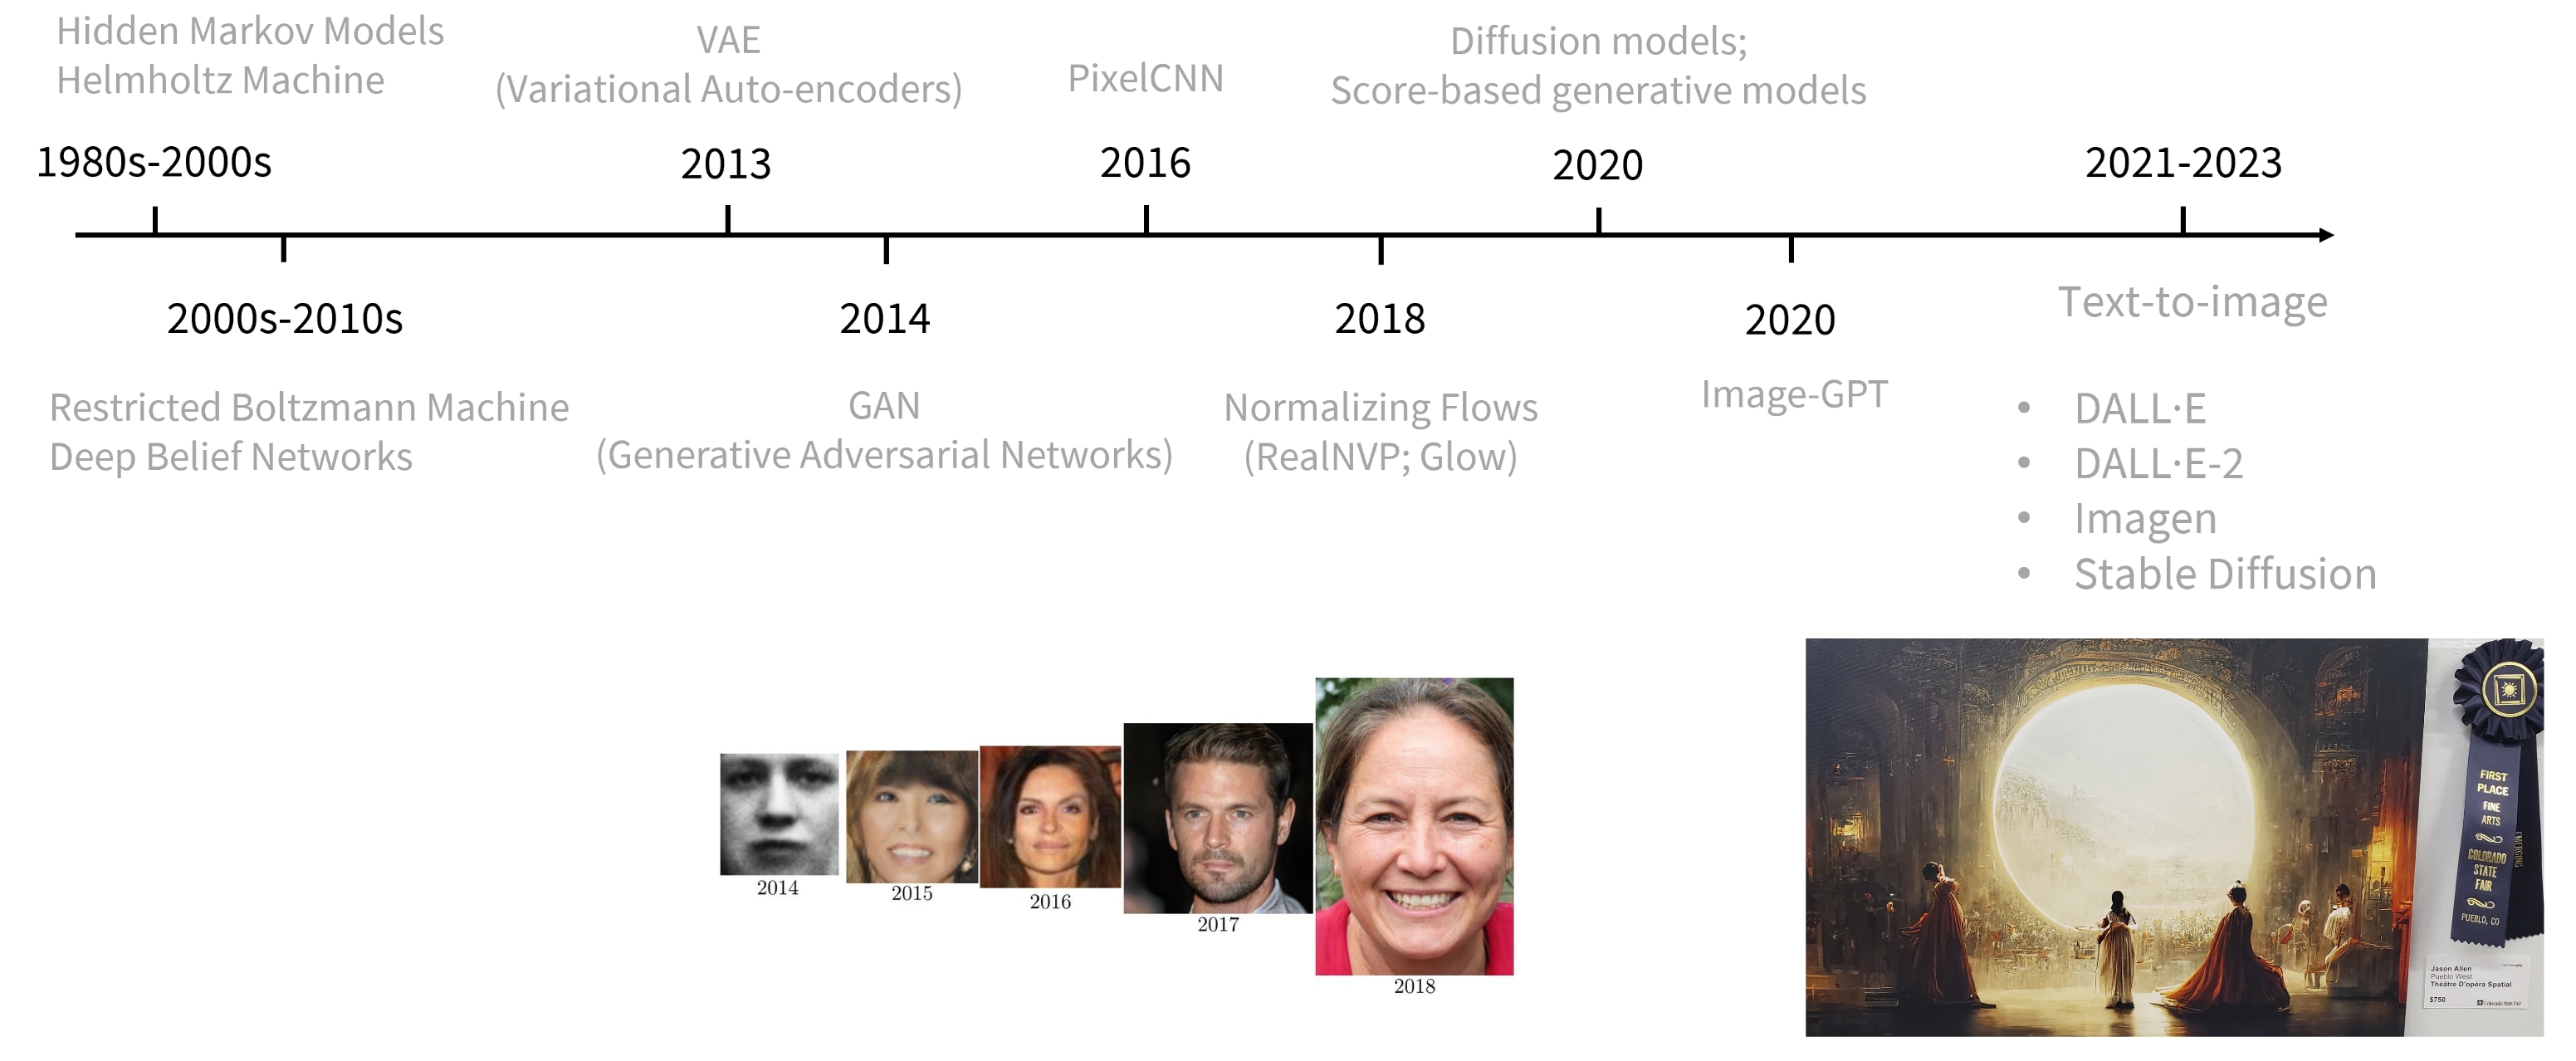
\includegraphics[width=0.95\linewidth]{genai_timeline.png}
      \caption{\scriptsize 生成式模型关键进展时间线~\parencite{dengPPTAdvancedNueralNetwork2024}。}
    \end{figure}
    \bottomleftrefs
  \end{frame}
  \end{refsection}



\begin{refsection}
  \begin{frame}
    \centering
    \vspace{2.5cm}
    {\LARGE \textbf{扩散模型:原理}}
  \end{frame}
\end{refsection}

\begin{refsection}
  \begin{frame}{去噪扩散模型}
  
    \begin{figure}
      \begin{minipage}{0.95\linewidth}
        \footnotesize
        \textbf{去噪扩散模型包含两个过程:}
        \begin{itemize}
          \item 正向扩散过程:逐步向输入中添加噪声。
          \item 反向去噪过程:通过去噪学习生成数据。
        \end{itemize}
      \end{minipage}
      \vspace{2em}
  
      \centering
      \includegraphics[width=1.0\linewidth]{diffusion_high_level.png}
  
      \caption[]{\scriptsize 扩散模型通过迭代去噪生成数据~\parencite{sohl2015deep,ho2020denoising}。 \scriptsize 图片来源:~\cite{CVPR2023Tutorial}。}
    \end{figure}
    \bottomleftrefs
  \end{frame}
\end{refsection}

\begin{refsection}
\begin{frame}{正向扩散过程}
  \footnotesize
  正向过程在 $T$ 步内的形式化定义:
  \begin{center}
    \includegraphics[width=1.0\linewidth]{tutorial_diffusion_1.png}
  \end{center}
  \vspace{-1em}
    
    \begin{align*}
      q(\mathbf{x}_t \mid \mathbf{x}_{t-1}) &= \mathcal{N}\left(\mathbf{x}_t; \sqrt{1-\beta_t}\,\mathbf{x}_{t-1}, \beta_t \mathbf{I}\right)
      \hspace{1.5em}
      \Longrightarrow
      \hspace{1.5em}
      q(\mathbf{x}_{1:T} \mid \mathbf{x}_0) = \prod_{t=1}^T q(\mathbf{x}_t \mid \mathbf{x}_{t-1})
      \hspace{1.5em}
      \text{\footnotesize (联合分布)}
    \end{align*}
  % \vspace{1em}
  \scriptsize 图片来源:~\cite{CVPR2023Tutorial}。
  \bottomleftrefs
  
\end{frame}
\end{refsection}

\begin{refsection}
\begin{frame}{扩散核}
  \begin{figure}
    \centering
    \includegraphics[width=1.0\linewidth]{diffusion_kernel.png}
  \end{figure}

  \vspace{-2em}

  {\small
  \begin{flushleft}
  \begin{align*}
    &\textbf{定义:} \qquad \overline{\alpha}_t = \prod_{s=1}^t (1 - \beta_s)
    &\implies q(\mathbf{x}_t \mid \mathbf{x}_0) = \mathcal{N}\left(\mathbf{x}_t; \sqrt{\overline{\alpha}_t}\, \mathbf{x}_0, (1 - \overline{\alpha}_t)\mathbf{I}\right) \hspace{1em} \text{\footnotesize (扩散核)}
  \end{align*}
  \end{flushleft}
  }
  \vspace{-1em}
  {\small
  \begin{flushleft}
  \begin{align*}
    &\textbf{采样公式:} \qquad \mathbf{x}_t = \sqrt{\overline{\alpha}_t}\, \mathbf{x}_0 + \sqrt{1 - \overline{\alpha}_t}\, \boldsymbol{\epsilon}
    &\text{其中} \quad \boldsymbol{\epsilon} \sim \mathcal{N}(\mathbf{0}, \mathbf{I})
  \end{align*}
  \end{flushleft}
  }

  \begin{flushleft}
  \footnotesize
  噪声调度 $\{\beta_t\}$ 的选择使得 $\overline{\alpha}_T \to 0$,且 $q(\mathbf{x}_T \mid \mathbf{x}_0) \approx \mathcal{N}(\mathbf{x}_T; \mathbf{0}, \mathbf{I})$。
  \end{flushleft}

  \scriptsize 图片来源:~\cite{CVPR2023Tutorial}。
  \bottomleftrefs
\end{frame}
\end{refsection}

\begin{refsection}
  \begin{frame}{正向扩散中分布会发生什么?}
      到目前为止,我们讨论了扩散核 $q(\mathbf{x}_t|\mathbf{x}_0)$,但 $q(\mathbf{x}_t)$ 呢?

      \vspace{1em}

        \centering
        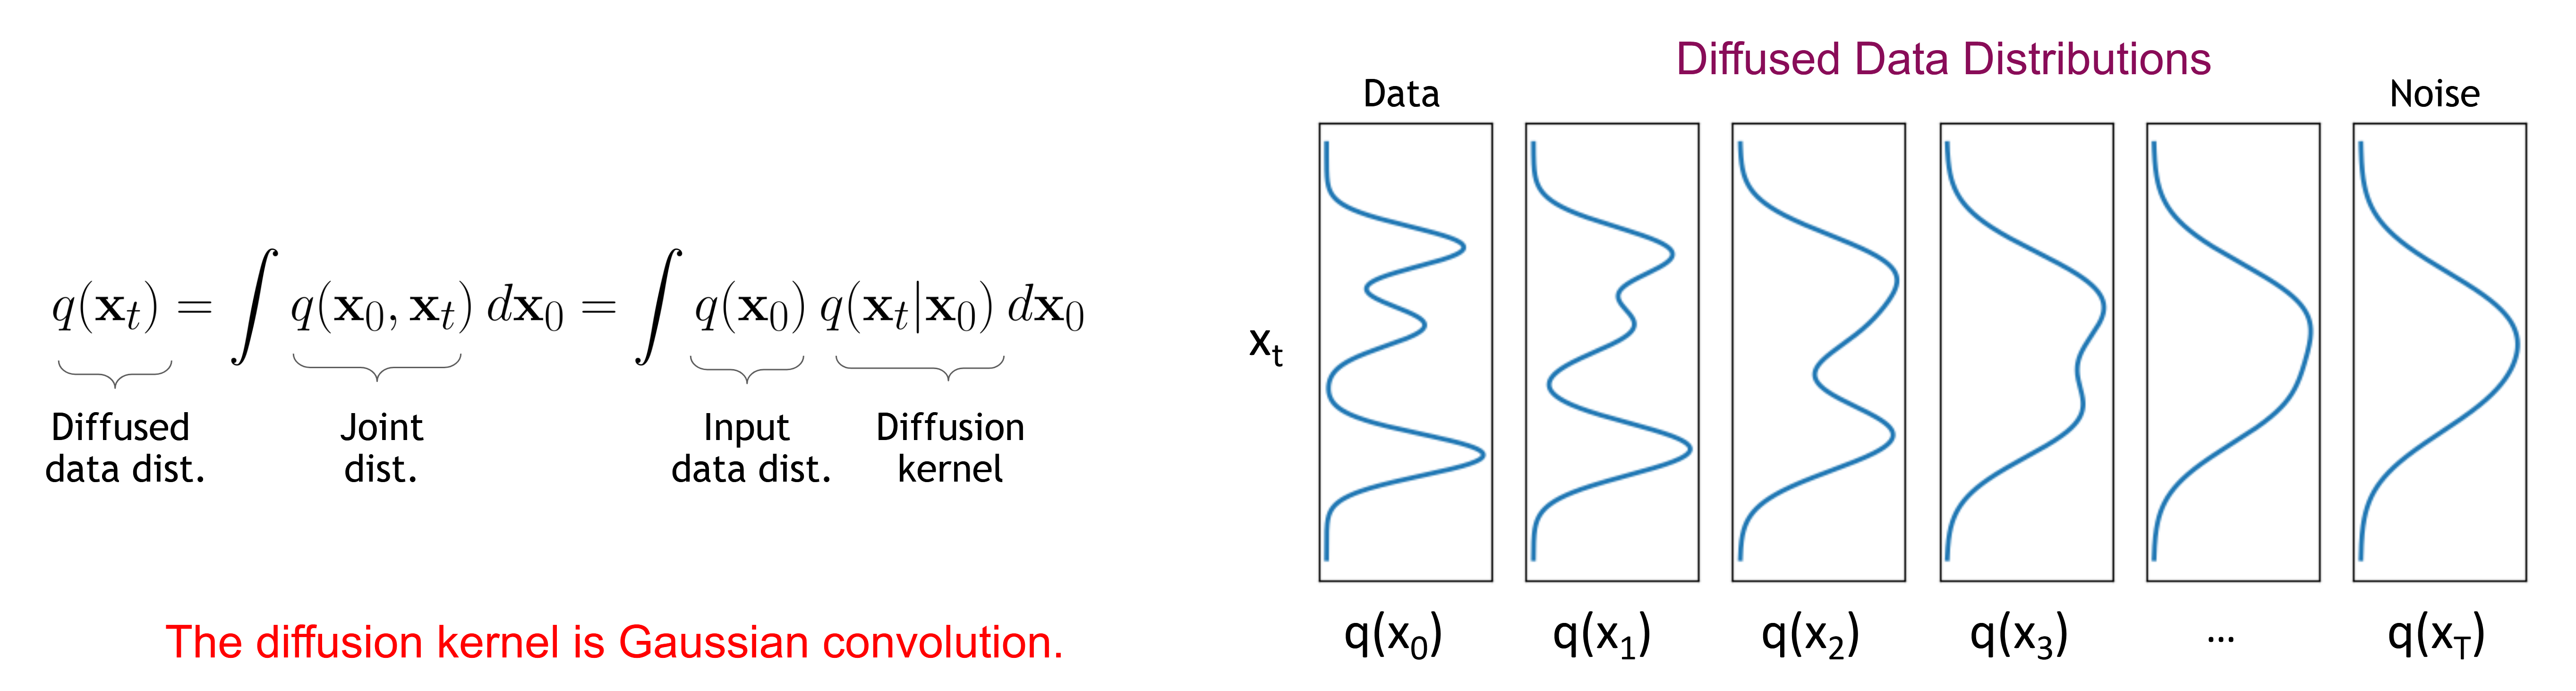
\includegraphics[width=\linewidth]{diffused_data_distributions.png}
  % \vspace{1em}

  
      我们可以先采样 $\mathbf{x}_0 \sim q(\mathbf{x}_0)$,再采样 $\mathbf{x}_t \sim q(\mathbf{x}_t|\mathbf{x}_0)$,从而得到 $\mathbf{x}_t \sim q(\mathbf{x}_t)$(即祖先采样)。
     
      \scriptsize 图片来源:~\cite{CVPR2023Tutorial}。
      \bottomleftrefs
  \end{frame}
  \end{refsection}


\begin{refsection}
\begin{frame}{通过去噪进行生成式学习}
  回顾:扩散参数被设计为 $q(\mathbf{x}_T) \approx \mathcal{N}(\mathbf{x}_T; 0, \mathbf{I})$。
  \begin{columns}
    \begin{column}{0.4\textwidth}
      \textbf{生成过程:}
      \begin{itemize}
        \item 采样 $\mathbf{x}_T \sim \mathcal{N}(\mathbf{x}_T; 0, \mathbf{I})$
        \item 迭代采样 $\mathbf{x}_{t-1} \sim \underbrace{q(\mathbf{x}_{t-1} \mid \mathbf{x}_t)}_{\text{真实去噪分布}}$
      \end{itemize}
    \end{column}
    \begin{column}{0.6\textwidth}
      \centering
      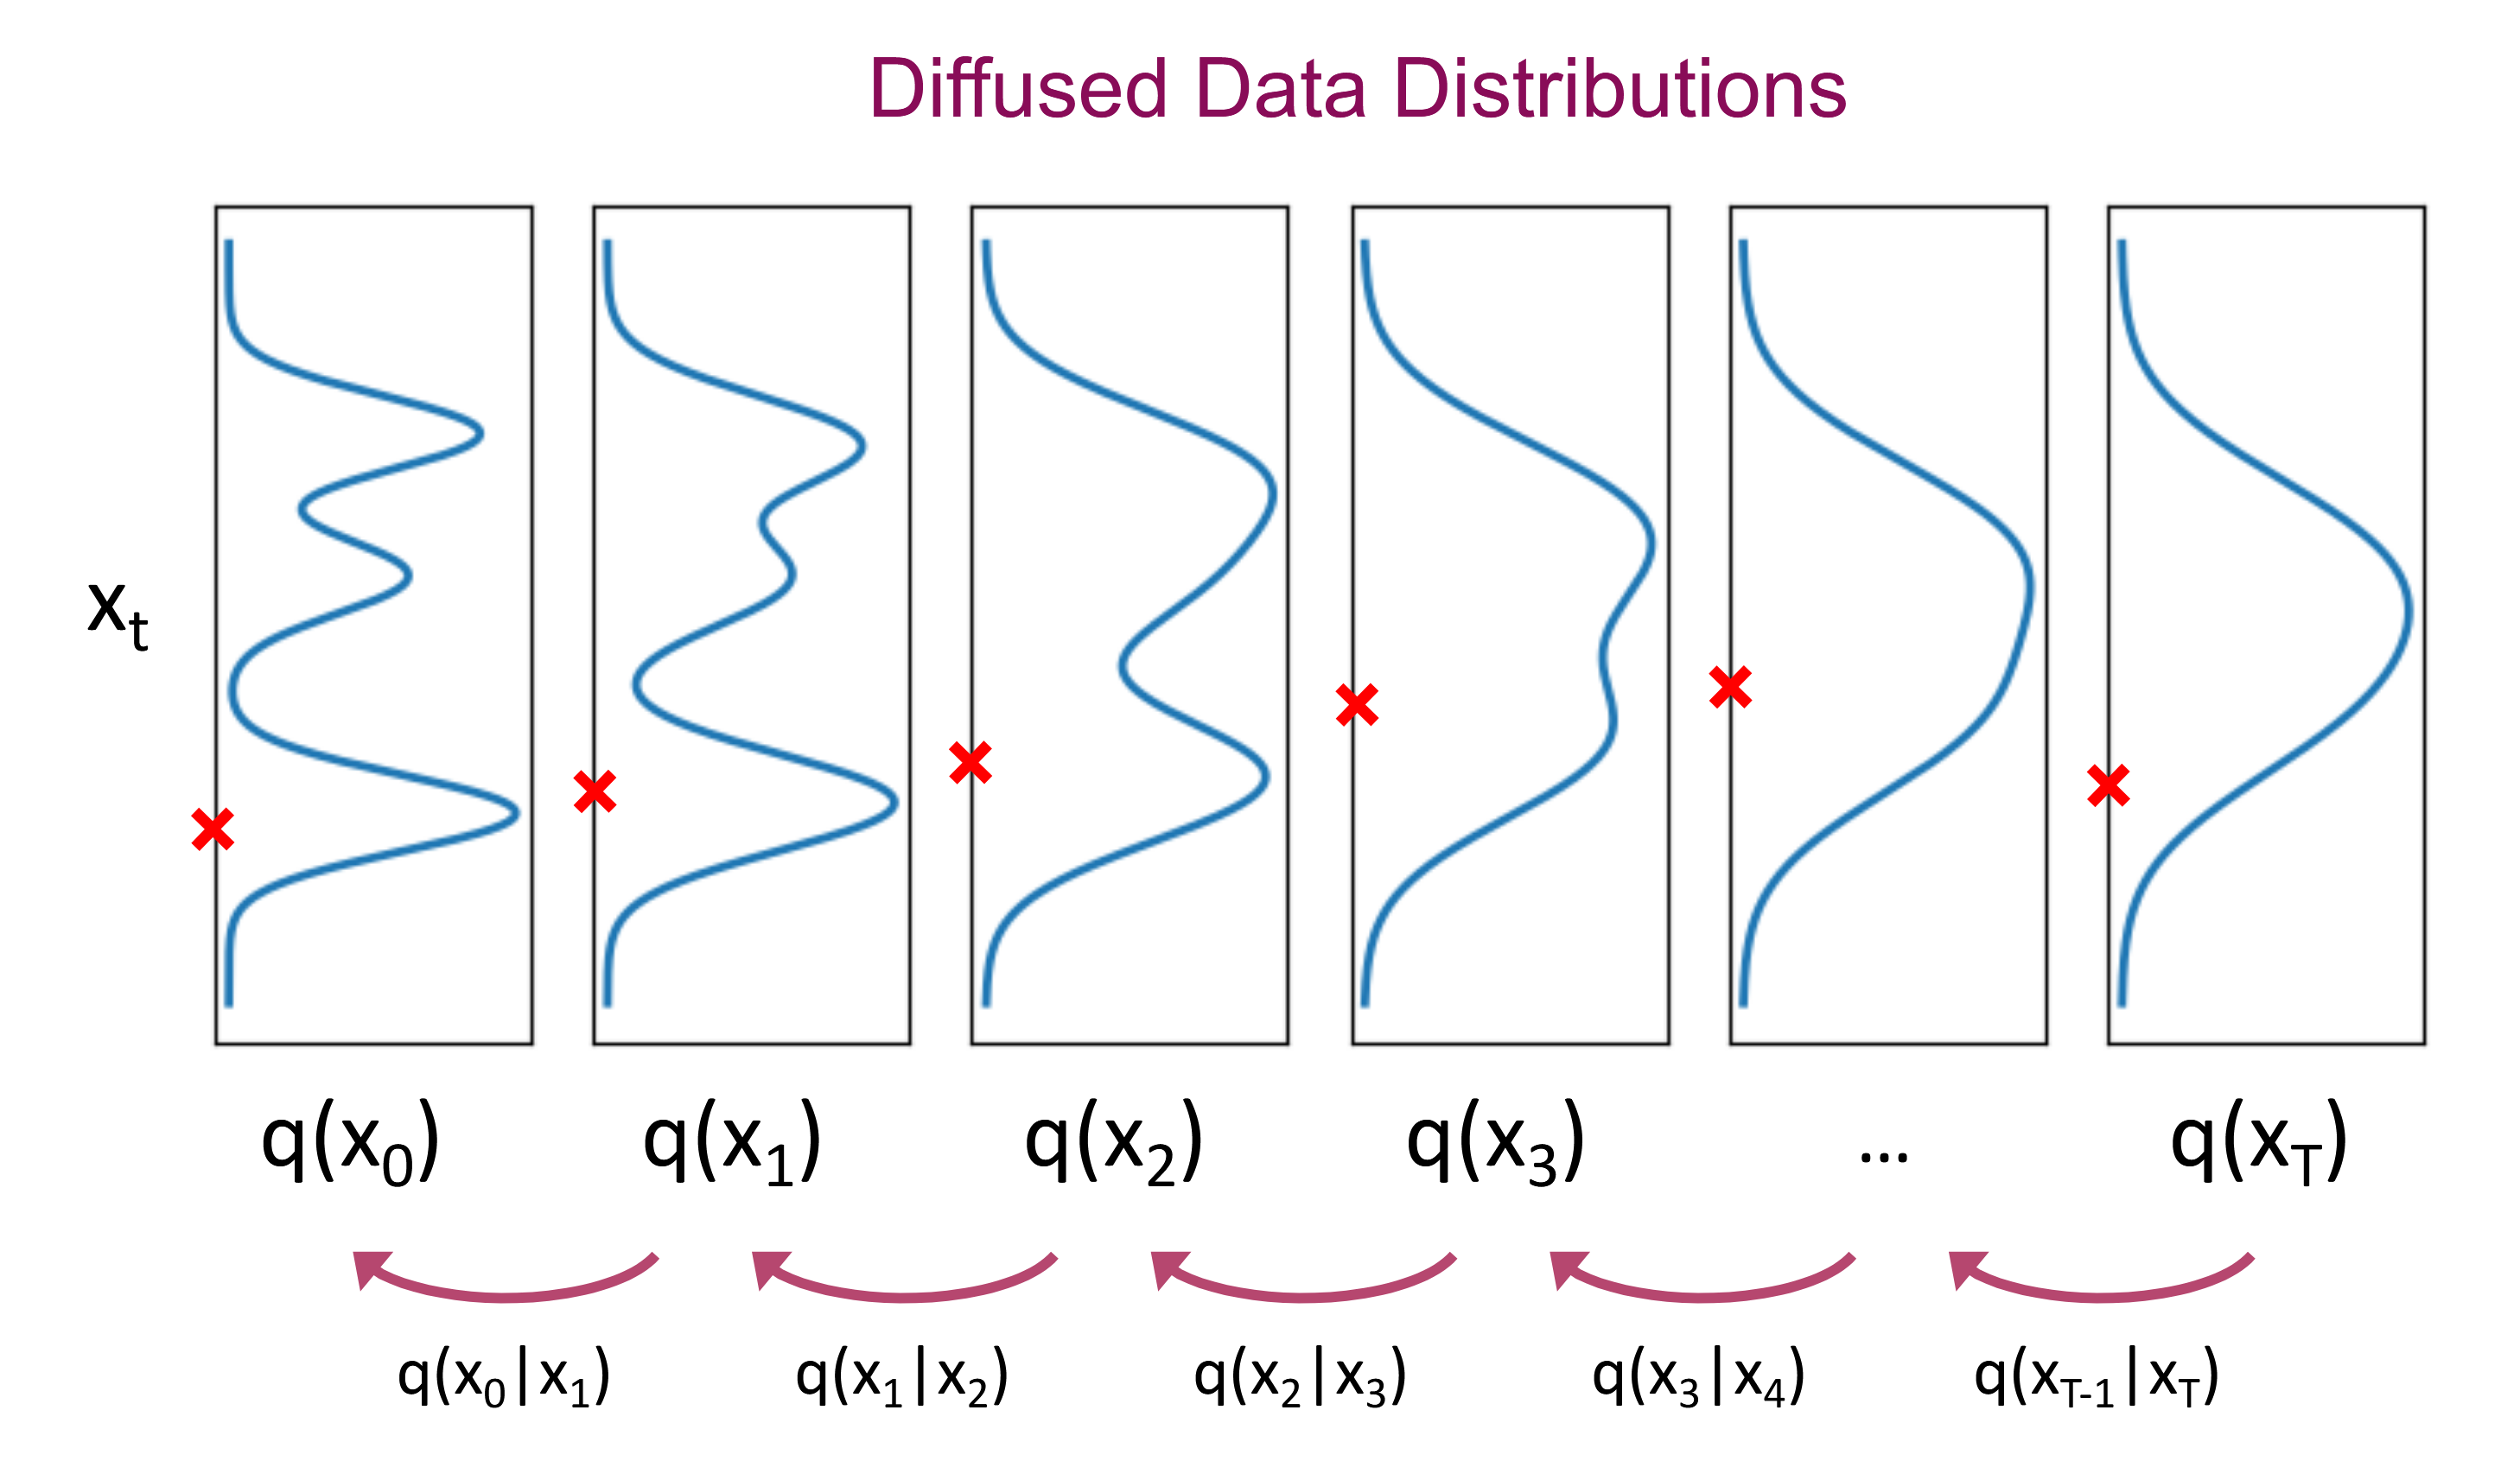
\includegraphics[width=1.0\linewidth]{generative_learning_by_denoising.png}
    \end{column}
  \end{columns}
  我们能否近似 $q(\mathbf{x}_{t-1} \mid \mathbf{x}_t)$?答案是可以的,如果每一步正向扩散中的 $\beta_t$ 很小,则可以用\textcolor{green}{高斯分布}近似。

  \scriptsize 图片来源:~\cite{CVPR2023Tutorial}。
  \bottomleftrefs
\end{frame}
\end{refsection}

\begin{refsection}
\begin{frame}{反向去噪过程}
  正向与反向过程在 $T$ 步内的形式化定义:
  \begin{center}
    \includegraphics[width=1.0\linewidth]{reverse_denoising_process.png}
  \end{center}
  \vspace{-2em}
  \begin{align*}
    p(x_T) &= \mathcal{N}(x_T; 0, I) \\
    p_\theta(x_{t-1}\mid x_t)
    &= \mathcal{N}\bigl(x_{t-1};\,\mu_\theta(x_t, t),\,\sigma_t^2 I\bigr)\quad
    \Rightarrow\quad
    p_\theta(x_{0:T})
    &= p(x_T)\,\prod_{t=1}^T p_\theta(x_{t-1}\mid x_t).
  \end{align*}
    \scriptsize
    其中 $\mu_\theta(x_t, t)$ 是可训练的神经网络(如 U-Net、去噪自编码器)

    \scriptsize 图片来源:~\cite{CVPR2023Tutorial}。
    \bottomleftrefs
\end{frame}
\end{refsection}

\begin{refsection}
\begin{frame}{去噪模型的学习}
  \begin{minipage}{1.0\linewidth}
  \centering
  {\color{purple}\scriptsize 变分上界}
  \vspace{0.3em}

  \begin{itemize}
    \setlength\itemsep{0.2em}
    \item {\scriptsize 训练时,采用变分上界(类似 VAE):}
    {\scriptsize
    \begin{align*}
      \mathbb{E}_{q_\lambda} [ \log p_\theta(\mathbf{x}) ] \leq \mathbb{E}_{q_\lambda} \left[ \log \frac{p_\theta(\mathbf{x}, \mathbf{z})}{q_\lambda(\mathbf{z}|\mathbf{x})} \right] = L
    \end{align*}
    }
    \item {\scriptsize $\mathbf{x}_t = \sqrt{\bar{\alpha}_t} \mathbf{x}_0 + \sqrt{1 - \bar{\alpha}_t} \boldsymbol{\epsilon}$,均值参数化方式见~\parencite{ho2020denoising}:}
    {\scriptsize
    \begin{align*}
      \mu_\theta(\mathbf{x}_t, t) = \frac{1}{\sqrt{\alpha_t}} \left( \mathbf{x}_t - \frac{1 - \alpha_t}{\sqrt{1 - \bar{\alpha}_t}} \boldsymbol{\epsilon}_\theta(\mathbf{x}_t, t) \right)
    \end{align*}
    }
    \item {\scriptsize 变分目标函数:}
    {\scriptsize
    \begin{align*}
      L = \mathbb{E}_{q(\mathbf{x}_0, \boldsymbol{\epsilon})} \left[ \sum_{t=1}^T \lambda_t \mathbb{E}_{q(\mathbf{x}_t|\mathbf{x}_0)} \left[ \left\| \boldsymbol{\epsilon} - \boldsymbol{\epsilon}_\theta(\sqrt{\bar{\alpha}_t} \mathbf{x}_0 + \sqrt{1 - \bar{\alpha}_t} \boldsymbol{\epsilon}, t) \right\|^2 \right] \right]
    \end{align*}
    }
    \item {\scriptsize 设置 $\lambda_t=1$ 对所有 $t$ 效果最佳~\parencite{ho2020denoising}。}
  \end{itemize}
  \end{minipage}
  \vspace{-0.5em}
  \bottomleftrefs
\end{frame}
\end{refsection}

\begin{refsection}
\begin{frame}{小结}
  \centering
  {\color{purple} \small 训练与采样过程}
  \vspace{1em}

  \begin{minipage}{0.45\linewidth}
    \scriptsize
    \textbf{Algorithm1-Training}
    \vspace{0.5em}
    \renewcommand{\arraystretch}{1.5}
    \begin{tabular}{l}
      \toprule
      1: \quad \textbf{重复} \\
      2: \quad \hspace{1em} $\mathbf{x}_0 \sim q(\mathbf{x}_0)$ \\
      3: \quad \hspace{1em} $t \sim \mathrm{Uniform}(\{1, \ldots, T\})$ \\
      4: \quad \hspace{1em} $\boldsymbol{\epsilon} \sim \mathcal{N}(0, I)$ \\
      5: \quad \hspace{1em} 对以下目标做梯度下降 \\
      \quad \hspace{2.5em} $\nabla_\theta \left\| \boldsymbol{\epsilon} - \boldsymbol{\epsilon}_\theta\left(\sqrt{\bar{\alpha}_t} \mathbf{x}_0 + \sqrt{1 - \bar{\alpha}_t} \boldsymbol{\epsilon}, t\right) \right\|^2$ \\
      6: \quad \textbf{直到收敛} \\
      \bottomrule
    \end{tabular}
  \end{minipage}
  \hfill
  \renewcommand{\arraystretch}{1.5}
  \begin{minipage}{0.45\linewidth}
    \scriptsize
    \textbf{Algorithm2-Sampling}
    \vspace{0.5em}
    \begin{tabular}{l}
      \toprule
      1: \quad $\mathbf{x}_T \sim \mathcal{N}(0, I)$ \\
      2: \quad \textbf{for} $t = T, \ldots, 1$ \textbf{do} \\
      3: \quad \hspace{1em} $\mathbf{z} \sim \mathcal{N}(0, I)$ \\
      4: \quad \hspace{1em} $\mathbf{x}_{t-1} = \frac{1}{\sqrt{\alpha_t}} \left( \mathbf{x}_t - \frac{1 - \alpha_t}{\sqrt{1 - \bar{\alpha}_t}} \boldsymbol{\epsilon}_\theta(\mathbf{x}_t, t) \right) + \sigma_t \mathbf{z}$ \\
      5: \quad \textbf{end for} \\
      6: \quad \textbf{return} $\mathbf{x}_0$ \\
      \bottomrule
    \end{tabular}
  \end{minipage}
  \renewcommand{\arraystretch}{1}
  \vspace{1em}

  算法来源:去噪概率扩散模型DDPM~\parencite{ho2020denoising}
  \bottomleftrefs
\end{frame}
\end{refsection}



\begin{refsection}
  \begin{frame}
    \centering
    \vspace{2.5cm}
    {\LARGE \textbf{遥感中的应用}}
  \end{frame}
\end{refsection}


\begin{refsection}
  \begin{frame}{DiffusionSat 简介}
    \begin{figure}
      \centering
      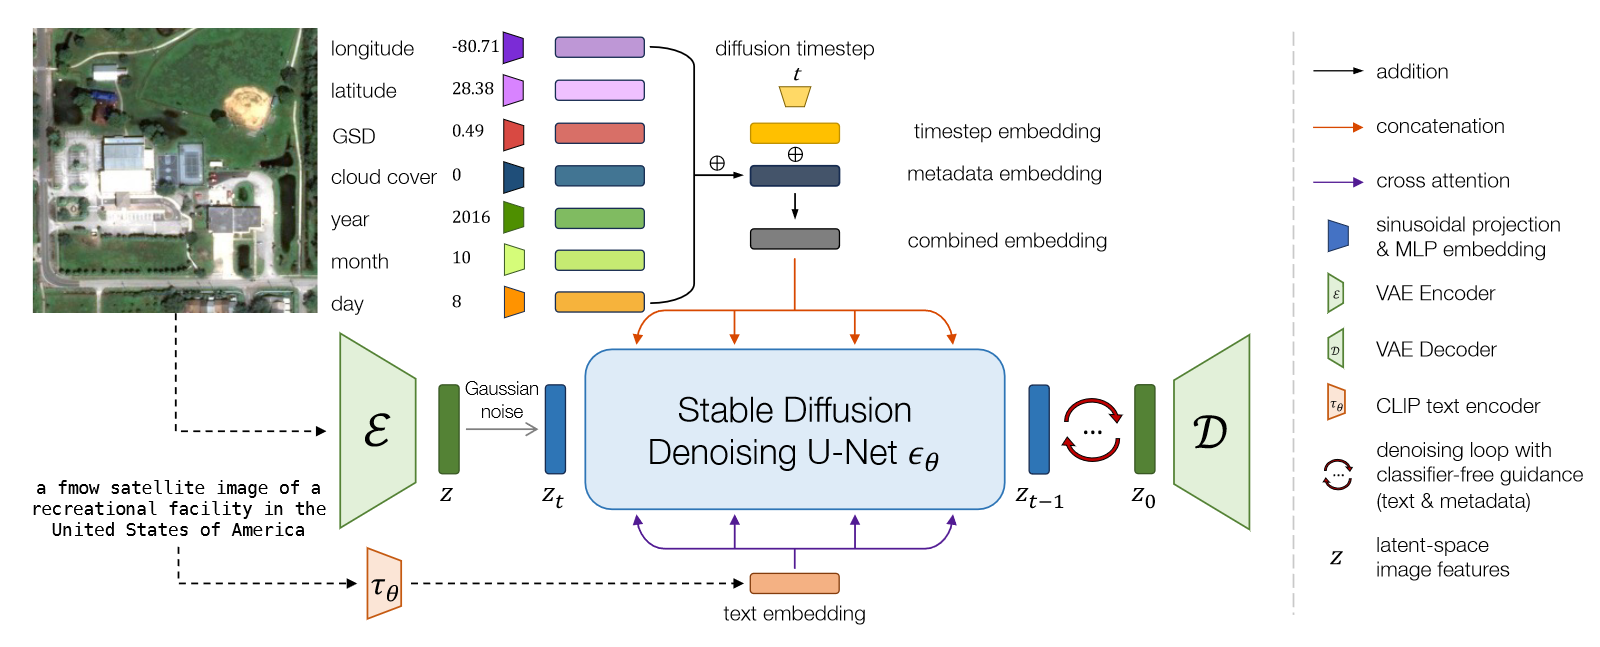
\includegraphics[width=0.85\linewidth]{diffusionsat_base.png}
      \caption{\scriptsize DiffusionSat \emph{base} 基础模型的整体架构,展示了如何将自由获取的元数据(传感器类型、日期、位置)与扩散主干网络融合,以生成高保真卫星影像~\parencite{diffusionset2024}。}
    \end{figure}
    \bottomleftrefs
  \end{frame}
\end{refsection}

\begin{refsection}
  \begin{frame}{DiffusionSat 的文本编码器}
    \begin{columns}[t]
      \begin{column}{0.4\textwidth}
        \small
        \begin{itemize}
          \item \textbf{输入提示:} \texttt{"A satellite image of a farmland"}
          \item \textbf{分词:}
          \begin{itemize}
            \item 拆分为子词 $\rightarrow$ token
            \item 示例映射: \(\{\text{"A"}:101,\ \text{" satellite"}:564,\ \dots,\ \texttt{<EOS>}:102\}\)
          \end{itemize}
          \item \textbf{CLIP 文本编码器:}
          \begin{itemize}
            \item Token ID $\rightarrow$ 512维嵌入
            \item 捕捉语义特征
          \end{itemize}
        \end{itemize}
      \end{column}
      \begin{column}{0.6\textwidth}
        \begin{figure}
          \centering
          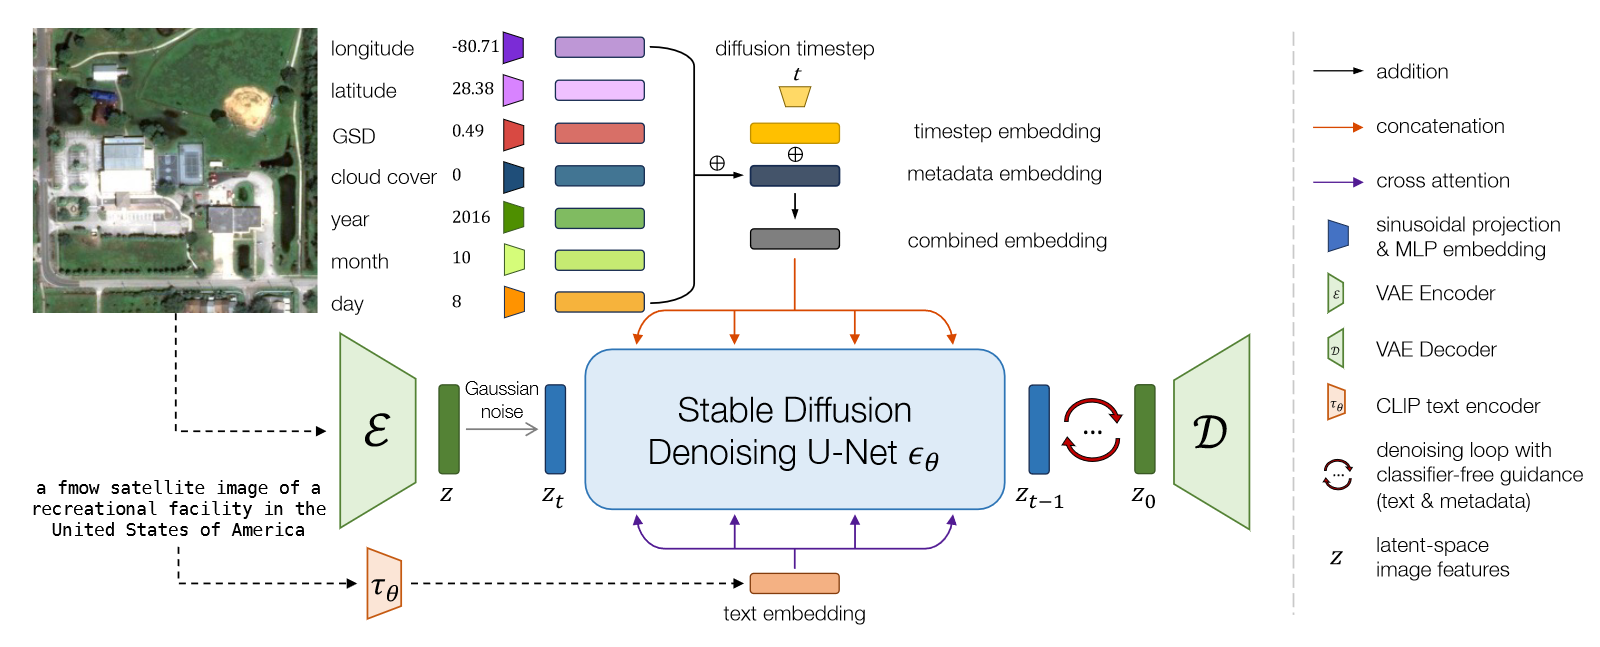
\includegraphics[width=1.0\linewidth]{diffusionsat_base.png}
          \caption{\scriptsize 文本编码器模块(OpenAI CLIP)对输入提示进行分词,并生成512维嵌入用于条件扩散主干网络~\parencite{diffusionset2024}。}
        \end{figure}
      \end{column}
    \end{columns}
    \bottomleftrefs
  \end{frame}
\end{refsection}

\begin{refsection}
  \begin{frame}{DiffusionSat 的元数据编码器}
    \begin{columns}[t]
      \begin{column}{0.4\textwidth}
        \small
        \begin{itemize}
          \item \textbf{输入元数据示例:}
          \begin{itemize}
            \item 传感器: Sentinel-2
            \item 位置: (纬度: 37.7749, 经度: -122.4194)
            \item 日期: 2022-06-01
            \item GSD: 10 m
            \item 云量: 5\%
          \end{itemize}
          \item \textbf{处理模块:} 元数据编码器
          \item \textbf{输出:} 512维条件嵌入
        \end{itemize}
      \end{column}
      \begin{column}{0.6\textwidth}
        \begin{figure}
          \centering
          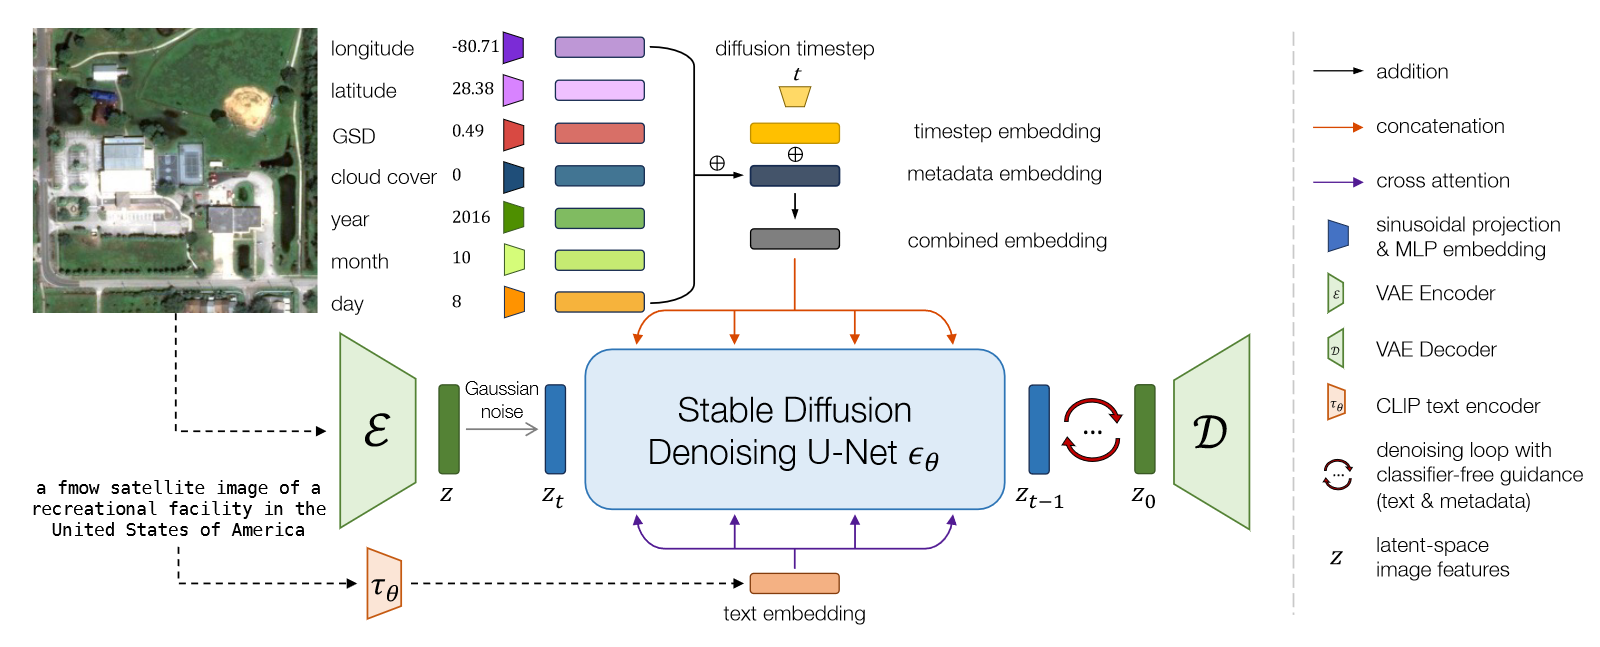
\includegraphics[width=1.0\linewidth]{diffusionsat_base.png}
          \caption{\scriptsize 元数据编码器将原始卫星元数据转换为定长嵌入,用于条件扩散主干网络~\parencite{diffusionset2024}。}
        \end{figure}
      \end{column}
    \end{columns}
    \bottomleftrefs
  \end{frame}
\end{refsection}

\begin{refsection}
  \begin{frame}{图像处理与扩散步骤}
    \begin{columns}[t]
      \begin{column}{0.5\textwidth}
        \small
        \begin{itemize}
          \item \textbf{训练流程:}
          \begin{itemize}
            \item 输入: 干净的卫星影像
            \item 编码: 图像编码器 $\rightarrow$ 隐变量
            \item 正向扩散: 在 \(T\) 步中加入高斯噪声
            \item 条件: 注入文本和元数据嵌入
            \item 学习: UNet 预测并去除噪声
          \end{itemize}
          \item \textbf{推理流程:}
          \begin{itemize}
            \item 输入: 随机噪声隐变量 \(x_T\!\sim\!\mathcal{N}(0,I)\)
            \item 反向扩散: 通过条件 UNet 迭代去噪
            \item 解码: 隐变量解码器 $\rightarrow$ 最终高保真影像
          \end{itemize}
        \end{itemize}
      \end{column}
      \begin{column}{0.5\textwidth}
        \begin{figure}
          \centering
          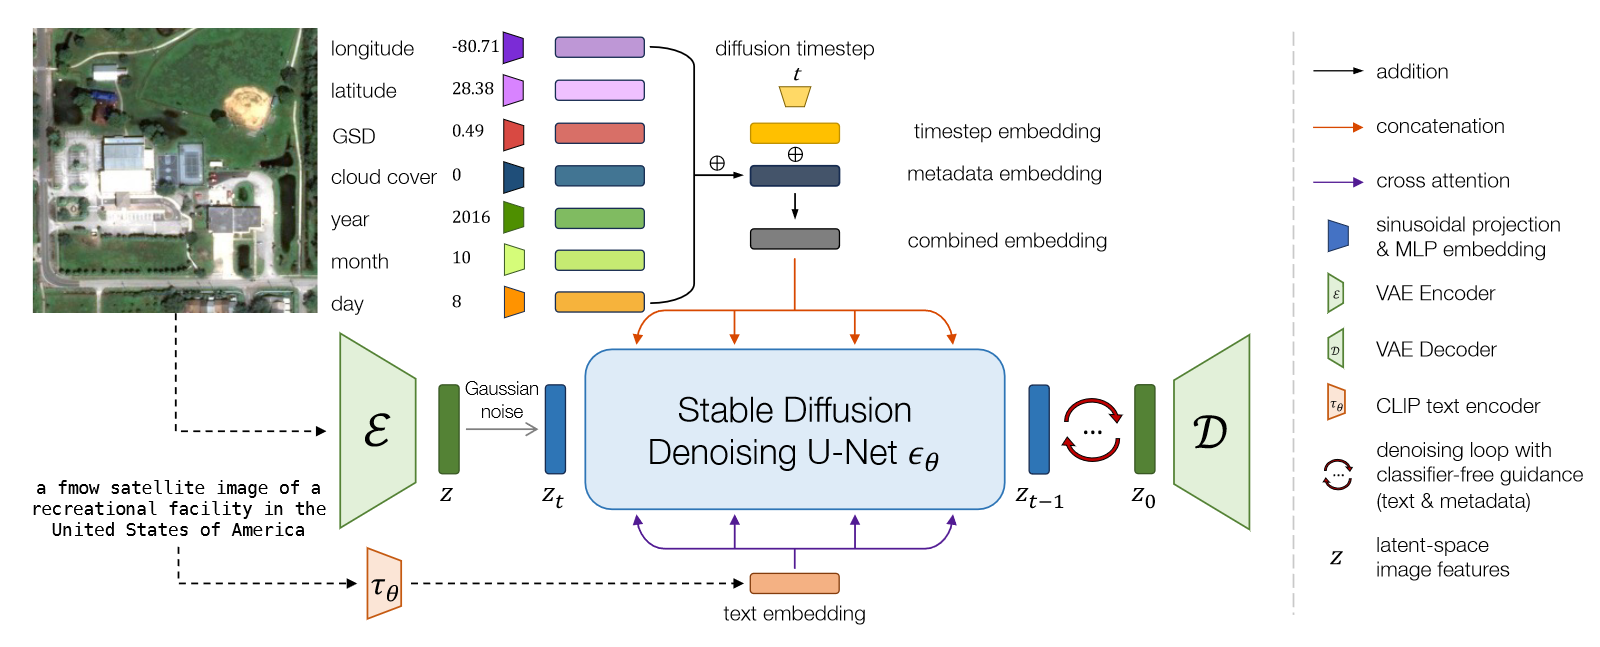
\includegraphics[width=1.0\linewidth]{diffusionsat_base.png}
          \caption{\scriptsize DiffusionSat 基础模型中训练(正向扩散)与推理(反向去噪)流程的对比,展示了影像如何经过编码器、扩散主干和解码器~\parencite{diffusionset2024}。}
        \end{figure}
      \end{column}
    \end{columns}
    \bottomleftrefs
  \end{frame}
\end{refsection}

\begin{refsection}
  \begin{frame}{反向扩散:采样}
    \begin{columns}[t]
      \begin{column}{0.4\textwidth}
        \small
        \begin{itemize}
          \item \textbf{生成:} \(x \sim p(\text{noise},\,c_{\text{text}},\,c_{\text{meta}})\)
          \item \textbf{其中:}
          \begin{itemize}
            \item noise: \(x_T\!\sim\!\mathcal{N}(0,I)\)
            \item \(c_{\text{text}}\): 文本(嵌入)
            \item \(c_{\text{meta}}\): 元数据(嵌入)
          \end{itemize}
        \end{itemize}
      \end{column}
      \begin{column}{0.6\textwidth}
        \begin{figure}
          \centering
          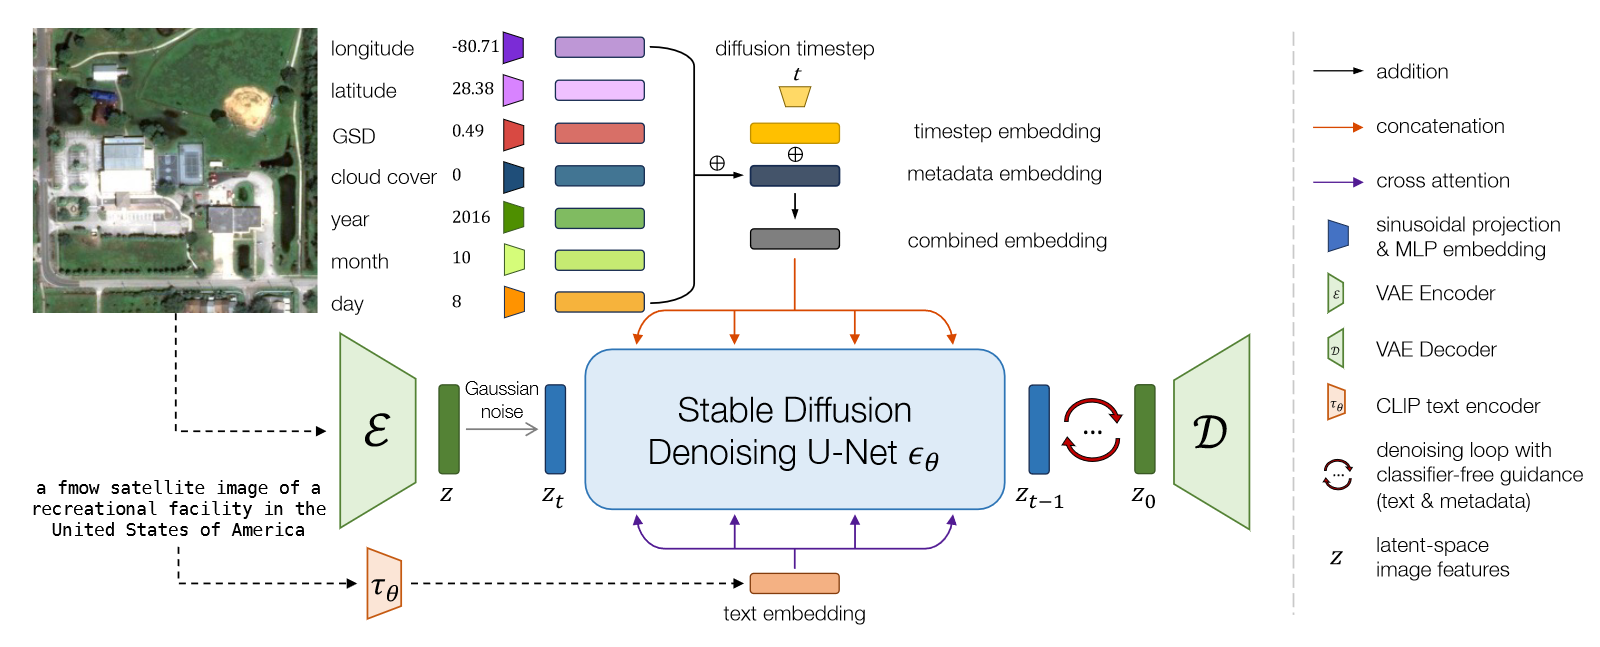
\includegraphics[width=1.0\linewidth]{diffusionsat_base.png}
          \caption{\scriptsize DiffusionSat 基础模型示意图~\parencite{diffusionset2024}。}
        \end{figure}
      \end{column}
    \end{columns}
    \bottomleftrefs
  \end{frame}
\end{refsection}
  

\begin{refsection}
  \begin{frame}{DiffusionSat+3DControlNet:框架概览}
    \begin{figure}
      \centering
      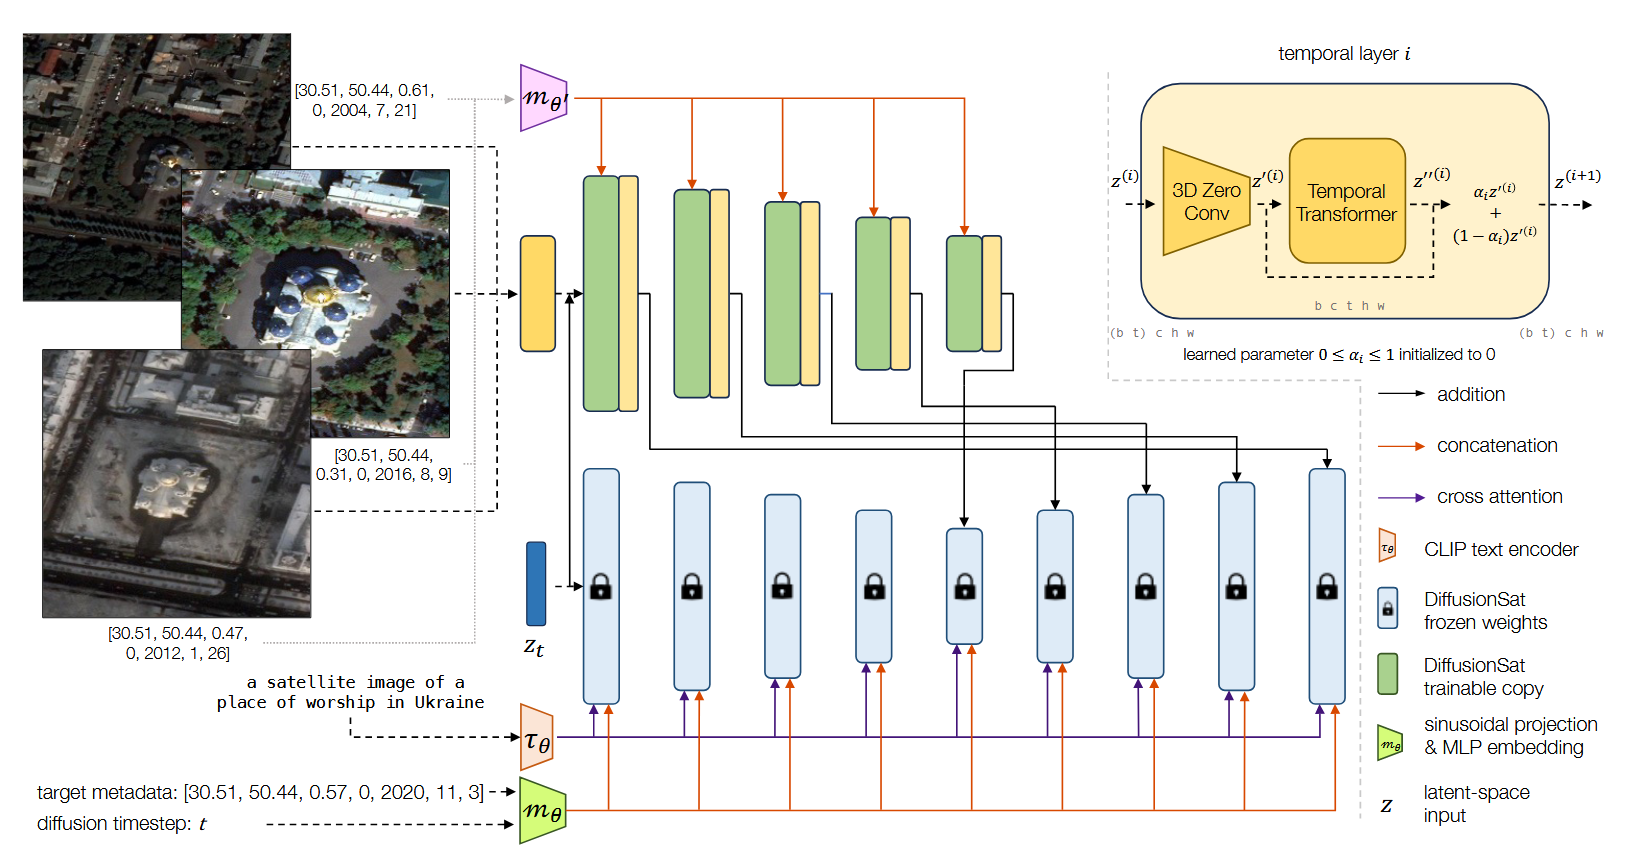
\includegraphics[width=0.9\linewidth]{diffusionsat.png}
      \caption[]{\scriptsize DiffusionSat 中的 3DControlNet。~\parencite{diffusionset2024}}
    \end{figure}
    \bottomleftrefs
  \end{frame}
\end{refsection}

\begin{refsection}
  \begin{frame}{DiffusionSat+3DControlNet: 时序预测结果}
    \begin{figure}
      \centering
      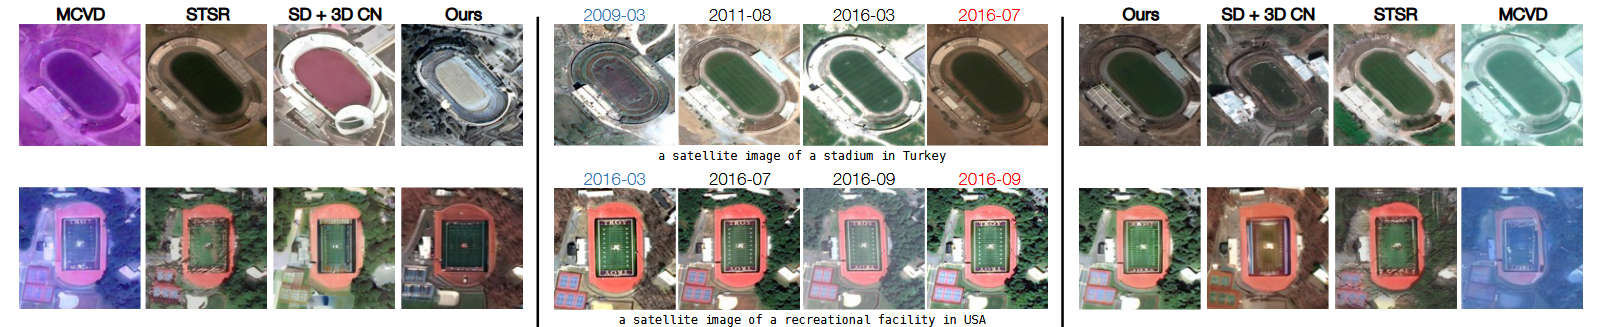
\includegraphics[width=1.0\linewidth]{diffusionsat_temporal_results.png}
      \caption[]{\scriptsize fMoW-temporal 数据集上的时序预测生成样例。~\parencite{diffusionset2024}}
    \end{figure}
    \begin{table}[h]
      \centering
      \scriptsize
      \begin{tabular}{l|ccc|ccc}
        \toprule
        \multirow{2}{*}{模型} & \multicolumn{3}{c|}{$t' > t$} & \multicolumn{3}{c}{$t' < t$} \\
        & SSIM$\uparrow$ & PSNR$\uparrow$ & LPIPS$\downarrow$ & SSIM$\uparrow$ & PSNR$\uparrow$ & LPIPS$\downarrow$ \\
        \midrule
        SD + 3D CN & 0.2027 & 11.0536 & 0.5523 & 0.2181 & 11.3004 & 0.5342 \\
        DiffusionSat + CN & 0.3297 & 13.6938 & 0.5062 & 0.2862 & 12.4990 & 0.5307 \\
        \textbf{DiffusionSat + 3D CN} & \textbf{0.3983} & \textbf{13.7886} & \textbf{0.4304} & \textbf{0.4293} & \textbf{14.8699} & \textbf{0.3937} \\
        \bottomrule
      \end{tabular}
      \caption[]{\scriptsize 表4:fMoW-temporal 验证集上的样本质量定量结果。$t' > t$ 表示已知未来影像生成过去影像,$t' < t$ 表示已知过去影像生成未来影像。}
    \end{table}
    \bottomleftrefs
  \end{frame}
\end{refsection}

\begin{refsection}
  \begin{frame}{DiffusionSat+3DControlNet:超分辨率结果}
    \begin{figure}
      \centering
      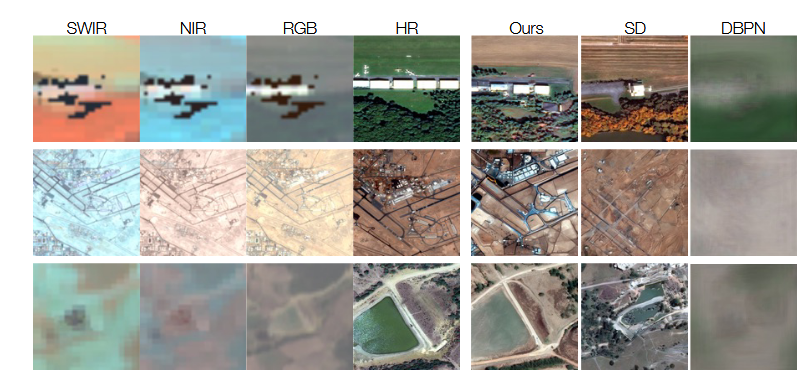
\includegraphics[width=0.9\linewidth]{diffusionsat_sr_results.png}
      \caption[]{\scriptsize DiffusionSat 在多光谱超分辨率任务中的示例结果。~\parencite{diffusionset2024}}
    \end{figure}
    \bottomleftrefs
  \end{frame}
\end{refsection}


\begin{refsection}
  \begin{frame}
    \centering
    \vspace{2.5cm}
    {\LARGE \textbf{进一步讨论}}
  \end{frame}
\end{refsection}

 
%--- 生成式模型用于数据增强 ---
\begin{refsection}
  \begin{frame}{利用生成式人工智能生成新图像}
    \begin{itemize}
      \item 生成式模型可以生成新的、逼真的图像。
      \item 我们可以用它们来扩充训练数据。
      \item 示例:给定“前”图像和描述,生成新的“后”图像。
    \end{itemize}
    \centering
    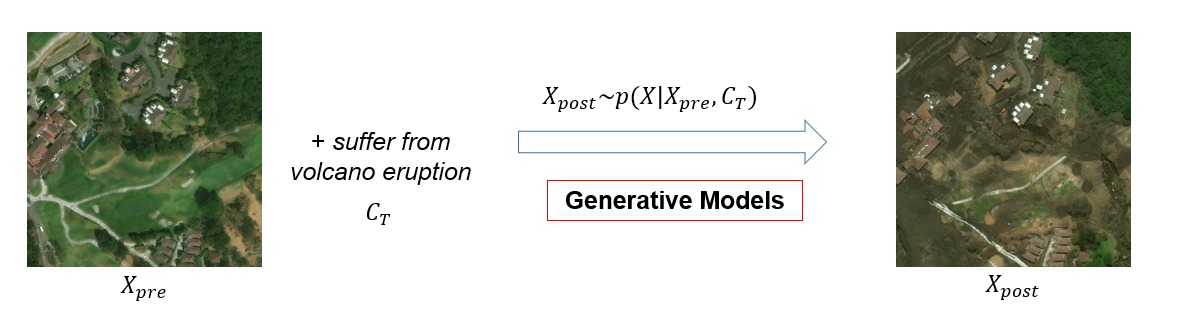
\includegraphics[width=1.0\linewidth]{diffusion_editing.png}
  \end{frame}
  \end{refsection}

  
\begin{refsection}
  \begin{frame}
    \centering
    \vspace{2.5cm}
    {\LARGE \textbf{补充内容}}
  \end{frame}
\end{refsection}

\begin{refsection}
  \begin{frame}{我们如何进行数据增强?}
    \textbf{经典方法:}
      \begin{itemize}
        \item 翻转、旋转、裁剪、改变颜色等。
      \end{itemize}
      \textbf{现代方法:}
      \begin{itemize}
        \item 融合两张图片(Mixup)~\parencite{zhangMixupEMPIRICALRISK2018}。
        \item 剪切并粘贴图片部分(CutMix)~\parencite{yunCutMixRegularizationStrategy2019}。
      \end{itemize}
    \begin{minipage}{0.58\linewidth}
      \begin{figure}
        \centering
        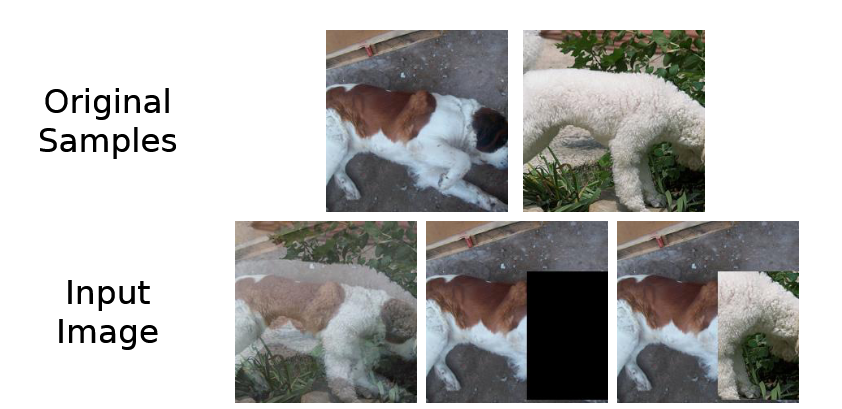
\includegraphics[width=0.6\linewidth]{aug_new_methods.png}
        \caption[]{\scriptsize 现代数据增强方法示意图。从左到右依次为:Mixup~\parencite{zhangMixupEMPIRICALRISK2018},Cutout~\parencite{devriesImprovedRegularizationConvolutional2017},CutMix~\parencite{yunCutMixRegularizationStrategy2019}。}
      \end{figure}
    \end{minipage}
    \hfill
    \begin{minipage}{0.4\linewidth}
      \textbf{软标签示例(CutMix):}
      % \vspace{0.5em}
      \tiny
      \begin{equation*}
        \text{cutmix\_label} = \lambda \cdot \text{label}_A + (1 - \lambda) \cdot \text{label}_B
      \end{equation*}
      \vspace{-0.5em}
      \begin{equation*}
        \text{示例:} \quad \lambda = 0.5, \quad \text{label}_A = [1, 0], \quad \text{label}_B = [0, 1]
      \end{equation*}
      \vspace{-0.5em}
      \begin{equation*}
        \text{cutmix\_label} = 0.5 \times [1, 0] + 0.5 \times [0, 1] = [0.5, 0.5]
      \end{equation*}
     
  
    \end{minipage}
    \bottomleftrefs
  \end{frame}
  \end{refsection}
  
  
\begin{refsection}
\begin{frame}{生成式模型用于数据增强}
  \begin{minipage}{0.7\linewidth}
    % \centering
    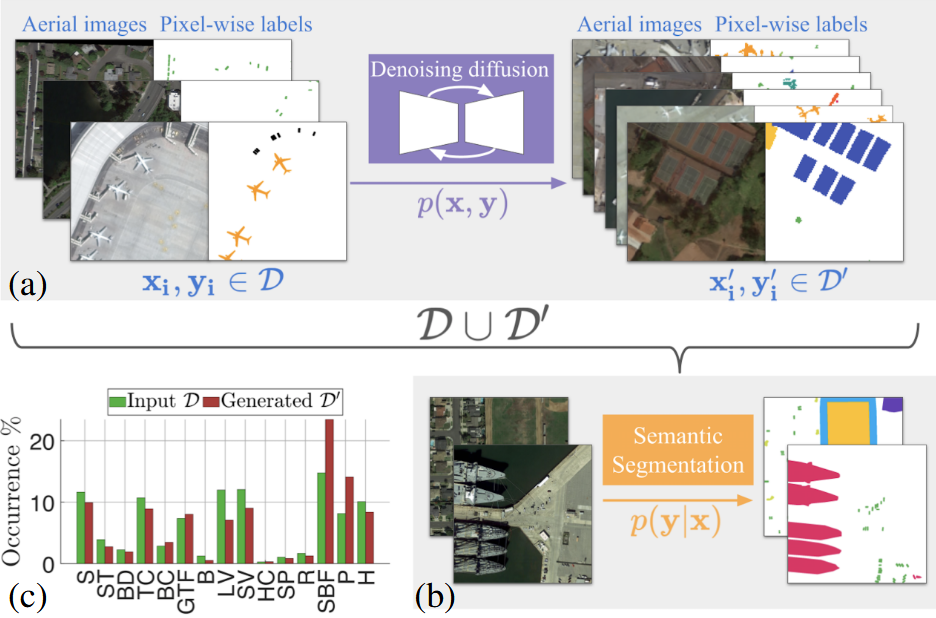
\includegraphics[width=0.9\linewidth]{satsyn.png}
  \end{minipage}%
  \hfill
  \begin{minipage}{0.3\linewidth}
    \scriptsize
    SatSyn~\parencite{tokerSatSynthAugmentingImageMask2024} 提出了一种生成式模型(扩散模型),可同时生成卫星分割的图像和对应掩码。该合成数据集用于数据增强,在卫星语义分割任务中,相比其他数据增强方法带来了显著的定量提升。
  \end{minipage}
  \bottomleftrefs
\end{frame}
\end{refsection}

\begin{refsection}
\begin{frame}{遥感图像生成中的应用:Text2Earth}
  \begin{figure}
    \centering
    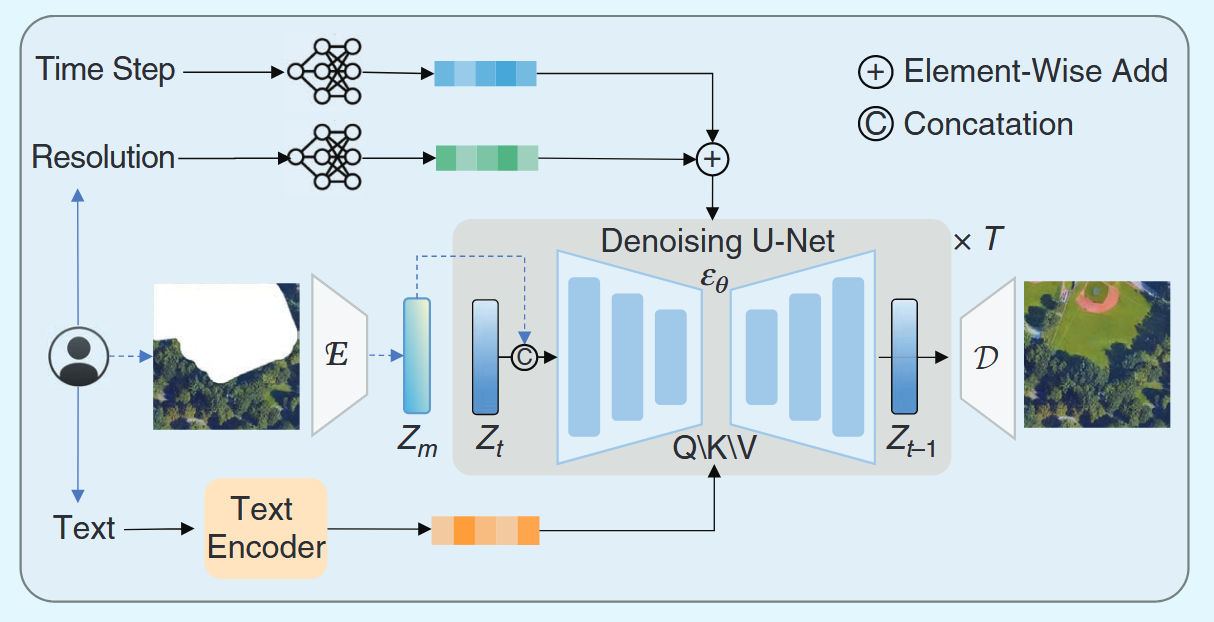
\includegraphics[width=0.9\linewidth]{text2earth.png}
    \caption[]{\scriptsize Text2Earth:面向文本驱动地球观测的基础模型~\parencite{text2earth2025}。}
  \end{figure}
  \bottomleftrefs
\end{frame}
\end{refsection}

\begin{refsection}
\begin{frame}{Text2Earth:示例结果}
  \begin{figure}
    \centering
    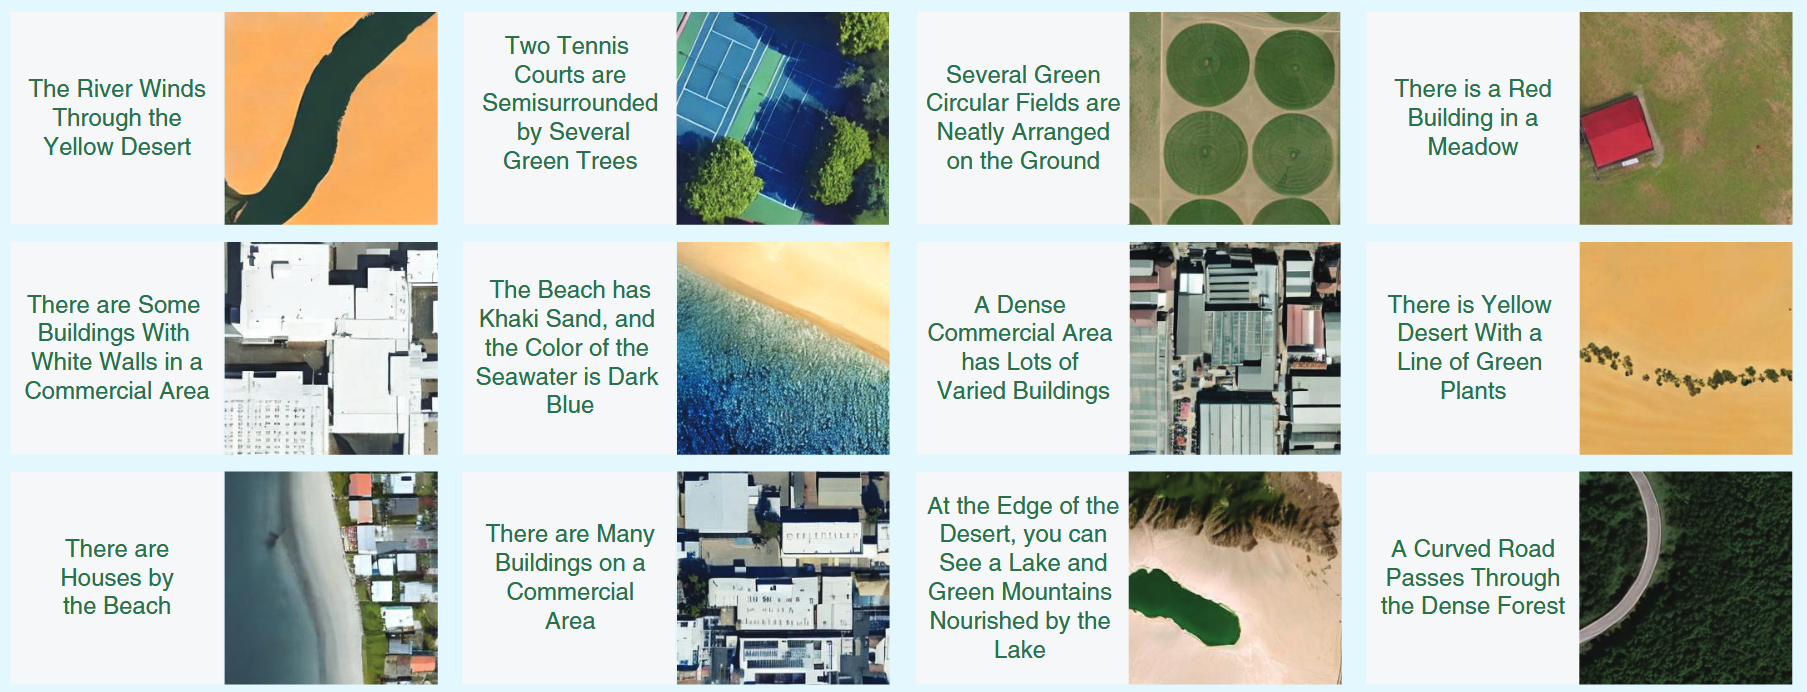
\includegraphics[width=0.9\linewidth]{text2earth_results.png}
    \caption[]{\scriptsize Text2Earth 生成的示例结果~\parencite{text2earth2025}。}
  \end{figure}
  \bottomleftrefs
\end{frame}
\end{refsection}

\begin{refsection}
\begin{frame}{遥感图像生成中的应用:CRS-Diff}
\begin{figure}
  \centering
  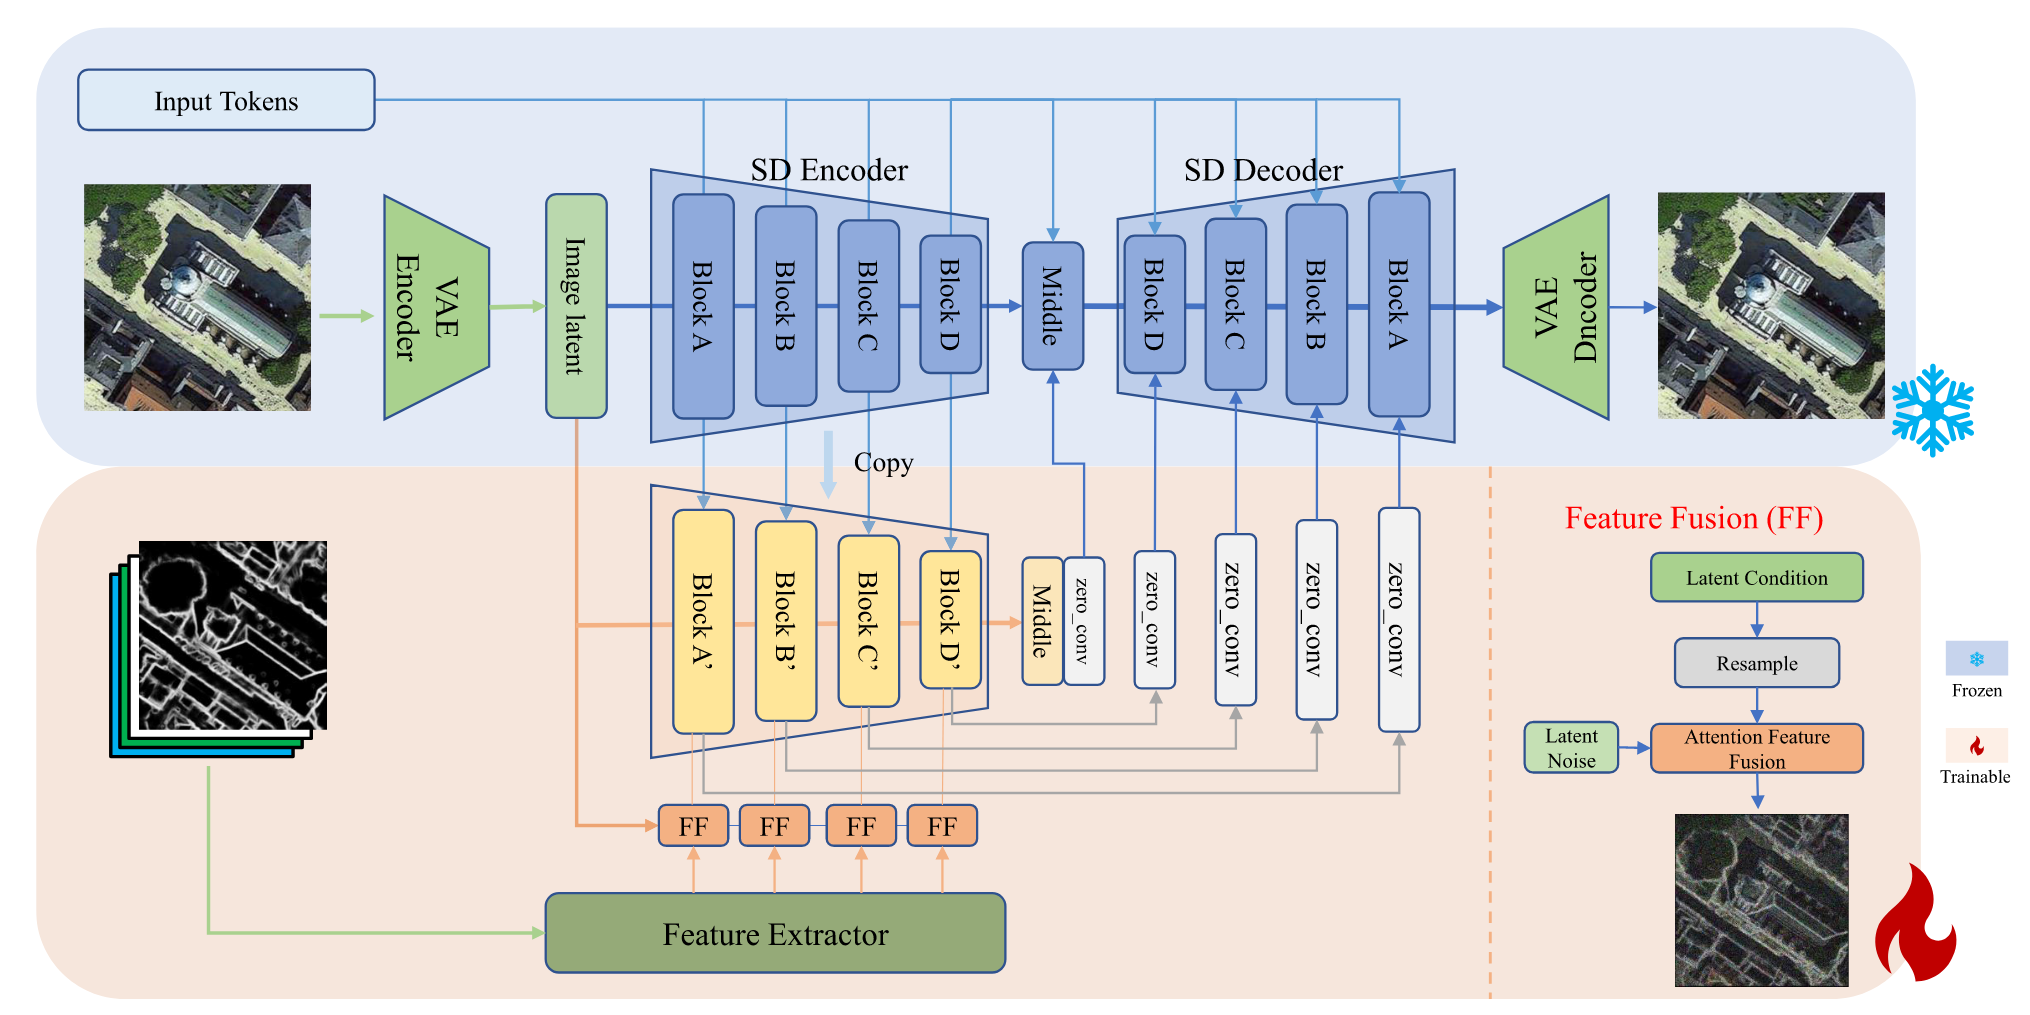
\includegraphics[width=0.9\linewidth]{crsdiff.png}
  \caption[]{\scriptsize CRS-Diff:可控遥感图像生成框架~\parencite{tang2024crsdiff}。}
\end{figure}
\bottomleftrefs
\end{frame}
\end{refsection}

\begin{refsection}
\begin{frame}{CRS-Diff:示例结果}
\begin{figure}
  \centering
  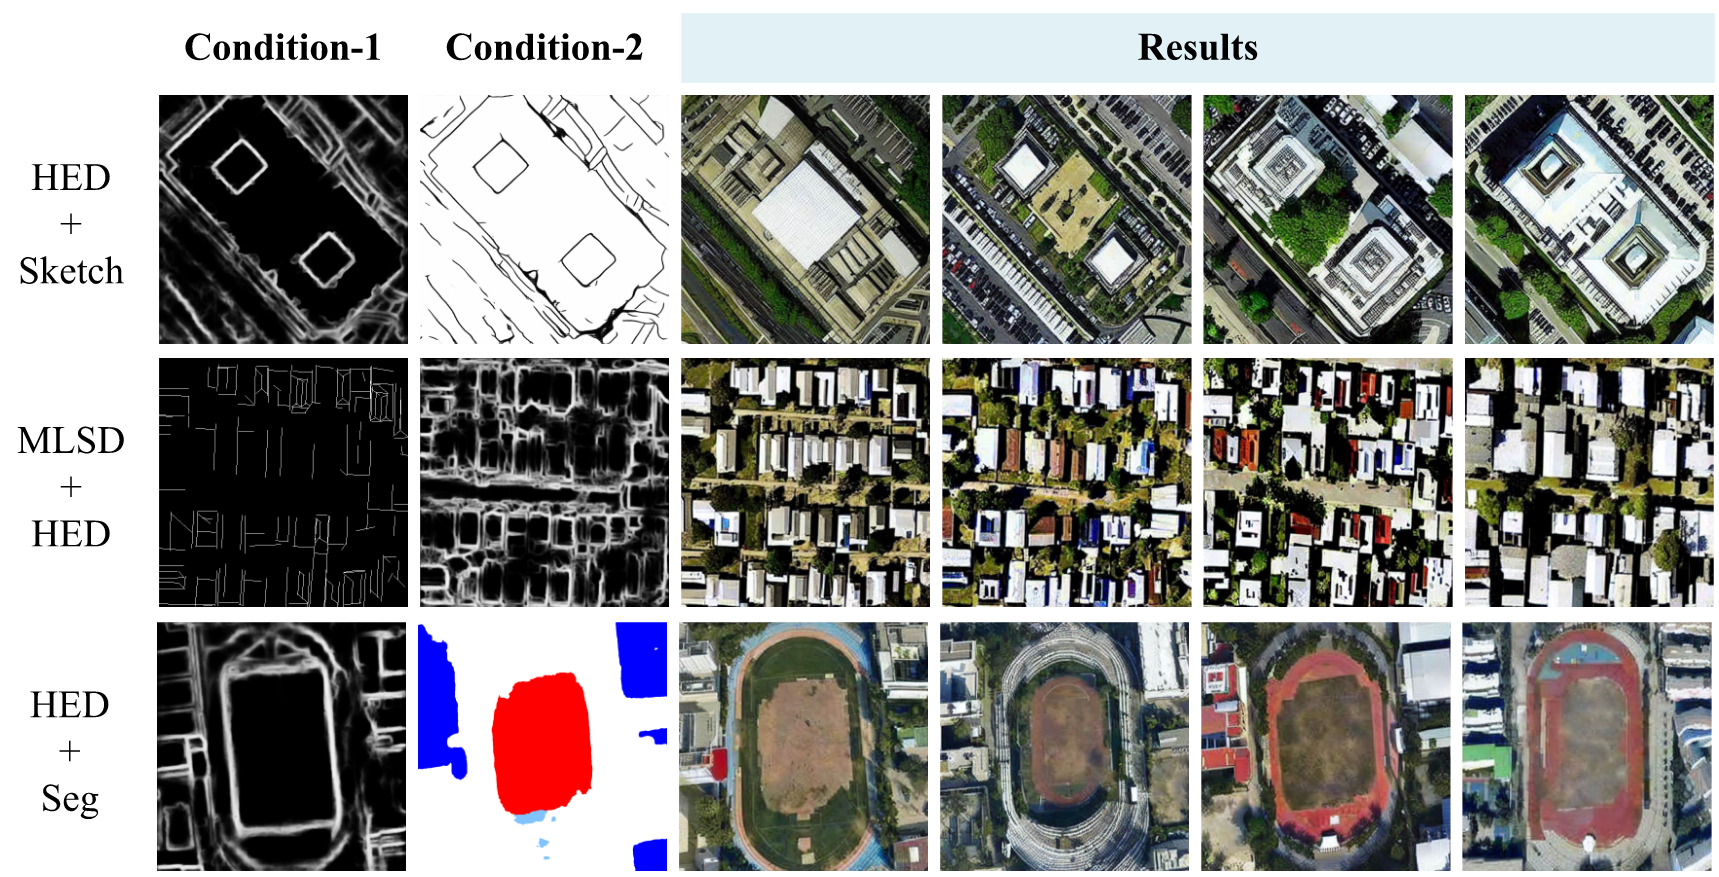
\includegraphics[width=0.9\linewidth]{crsdiff_results.png}
  \caption[]{\scriptsize CRS-Diff 生成的示例结果~\parencite{tang2024crsdiff}。}
\end{figure}
\bottomleftrefs
\end{frame}
\end{refsection}